\documentclass[a4paper,12pt]{article}
\usepackage[polish]{babel}
\usepackage[T1]{fontenc}
\usepackage[utf8]{inputenc}
\usepackage{mathtools, graphicx, float}
\title{Implementacja odległości Levenshteina w języku JavaScript}
\author{Jakub Piśkiewicz}
\date{\today}
\setlength{\parskip}{1em}
\graphicspath{ {./media} }
\begin{document}
\maketitle

\section{Terminologia}
W tym tekście użyto pewnych terminów, które mogą wymagać krótkiego objaśnienia.
\begin{itemize}
    \item słowo - ciąg zera lub więcej znaków. Nie musi mieć żadnego sensu.
    \item string - w języku angielskim oznacza ciąg znaków. Nazwa bardzo często używana w językach programistycznych.
\end{itemize}

\section{Różne typy miar odległości między słowami}
Odległość między słowami to najmniejsza możliwa 
liczba operacji wymaganych aby przejść z jednego słowa w drugie.
Odległość Levenshteina jest jednym czterech typów pomiarów odległości
między słowami. Typy pomiarów odległości różnią się między
sobą operacjami na słowach ze sobą porównywanych. \cite{wiki::edit}
Dla odległości Levenshteina operacje proste na słowach to:
\textbf{wstawienie} nowego znaku do słowa, 
\textbf{usunięcie} znaku ze słowa lub
\textbf{zamiana} znaku w słowie na inny. \cite{wiki::levenshteinpl}

\section{Opis miary odległości Levenshteina}
\subsection{Operacje proste na słowach i ich przykłady}
Tabela 1 przedstawia wszystkie operacje proste według miary odległości
Levenshteina i przykład ich działania na słowie "helikopter".

\begin{center}
    \begin{tabular}{|c|c|}
        \hline
        nazwa operacji      &       przykład działania\\
        \hline
        wstawianie          &       helikopter \( \rightarrow \) helikoptera\\
        \hline
        usuwanie            &       helikopter \( \rightarrow \) helikopte\\
        \hline
        zamiana             &       helikopter \( \rightarrow \) helikoptur\\
        \hline
    \end{tabular}

    \vspace{12pt}
    Tabela 1 - operacje proste i ich przykłady.
\end{center}

Działanie operacji prostych można także przedstawić w poniższy
sposób na przykładzie słowa \( A = uv \). Znak \( \varepsilon \) oznacza pusty string. \cite{wiki::edit}
\begin{itemize}
    \item wstawianie - \( A = uxw, \; \varepsilon \rightarrow x \)
    \item usuwanie - \( A = uv, \; x \rightarrow \varepsilon \)
    \item zamiana - \( A = vv, \; u \rightarrow v \)
\end{itemize}

\subsection{Koszty operacji na słowach}
W wielu odmianach miar odległości między słowami każda z operacji
elementarnych ma swój koszt. W przypadku odległości Levenshteina
koszty operacji wstawiania i usuwania jednego znaku wynoszą 1.
Koszt zamiany znaku na taki sam wynosi 0, natomiast koszt zamiany
na znak inny wynosi 1.

\subsection{Przykład}
Odległość Levenshteina między słowami \( A \) = "'silnik"' i \( B \) = "'wirnik"'
wynosi 2.
W celu porównania obu słów należy wykonać następujące
transformacje:

\begin{enumerate}
    \item \textbf{s}ilnik \( \rightarrow \) \textbf{w}ilnik
          - koszt operacji zamiany wynosi 1 (s \( \rightarrow \) w).
    \item s\textbf{i}lnik \( \rightarrow \) w\textbf{i}rnik
          - koszt zamiany i na i jest zerowy.
    \item wi\textbf{l}nik \( \rightarrow \) wi\textbf{r}nik
          - koszt zamiany \( ( l \rightarrow r ) \) jest równy 1, wobec czego odległość wzrasta do 2.
    \item wir\textbf{n}ik \( \rightarrow \) wir\textbf{n}ik
          - koszt zamiany n na n jest zerowy, więc odległość nie zmienia się.
    \item wirn\textbf{i}k \( \rightarrow \) wirn\textbf{i}k - koszt operacji = 0. Odległość bez zmian.
    \item wirni\textbf{k} \( \rightarrow \) wirni\textbf{k} - odległość między słowami = 2.
\end{enumerate}

Ostatecznie odległość między tymi słowami wyniosła 2, ponieważ jedynymi operacjami
prostymi, których koszt \( > 0 \) wymaganymi do przejścia ze słowa \( A \) w słowo \( B \)
były dwie operacje zamiany: s \( \rightarrow \) w i l \( \rightarrow \) r.

Ciekawostka - odległość Hamminga jest możliwa do obliczenia dla tych dwóch
słów, ponieważ są one identycznej długości. Wyniosła by ona tyle samo
co odległość Levenshteina, ponieważ jedynym typem operacji
potrzebnym do przejścia z jednego słowa w drugie jest zamiana.
Zamiana jest jedynym typem operacji dozwolonym w odległości Hamminga.
W przypadku gdy słowa są takiej samej długości górną granicą ich
odległości w metryce Levenshteina jest ich wzajemna odległość
według metryki Hamminga.

\subsection{Właściwości}
Każda miara odległości z kosztami operacji \( > 0 \)
i możliwością cofnięcia każdej operacji za tym samym kosztem
(na przykład koszt usunięcia znaku jest taki sam jak
koszt wstawienia tego znaku) może być uznawana za metrykę
pod warunkiem spełnienia następujących warunków:
\begin{itemize}
    \item Odległość między tymi samymi słowami wynosi 0.
    \item Odległość między różnymi od siebie słowami jest
          wyższa od 0, ponieważ co najmniej jedna operacja o koszcie
          większym od 0 potrzebna jest do przyrównania tych słów
          do siebie.
    \item Dla trzech słów: \( A \), \( B \) oraz \( C \): \( d(A,C) \le d(A,B) + d(B,C) \).
          Gdzie \( d(x,y) \) oznacza odległość międzdy słowami \( x \) i \( y \).
          Czyli zachodzi nierówność trójkątna.
\end{itemize}

Taka metryka tworzy wraz ze słowami dla których określa ona
odległość - przestrzeń metryczną. Przestrzeń metryczna to
zbiór z zadaną na nim funkcją określającą odległość między jego
elementami. \cite{wiki::metricpl}

Odległość Levenshteina spełnia te aksjomaty wobec czego jest to
metryka.

\subsection{Definicja}
Aby stworzyć algorytm wykorzystujący metrykę odległości Levenshteina
należy spojrzeć na jej definicję. \cite{wiki::levenshteinen}

\begin{equation*}
    lev(a,b) = \begin{cases}
        |a| & \text{jeżeli} \; |b| = 0,\\
        |b|  & \text{jeżeli} \; |a| = 0,\\
        lev(tail(a), tail(b)) & \text{jeżeli} \; a[0] = b[0]\\
        1 + min \begin{cases}
            lev(tail(a), b)\\
            lev(a, tail(b)) & \text{w innym wypadku}\\
            lev(tail(a), tail(b))
        \end{cases}
    \end{cases}
\end{equation*}

\( |x| \) oznacza długość słowa \( x \). \( x[i] \) oznacza i-ty znak
w słowie \( x \).

W definicji znajduje się kilka kluczowych informacji o działaniu
algorytmu:
\begin{itemize}
    \item Jeżeli jedno ze słów zawiera zero znaków. Odległością Levenshteina jest długość drugiej sekwencji.
    \item W przypadku gdy pierwszy znak w obydwu słowach jest taki sam,
          funkcja \( lev(a,b) \) jest wywoływana rekursywnie dla obydwu słów
          bez znaku pierwszego.
    \item Jeżeli długości słów są większe od 0 i pierwszy znak nie jest
          taki sam, wynik przyjmuje wartość najmniejszą spośród rekursywnych
          wywołań pomiaru odległości Levenshteina odpowiednio dla operacji
          wstawiania - \( lev(tail(a), b) \), usuwania - \( lev(a, tail(b)) \)
          i zamiany - \( lev(tail(a), tail(b)) \).
\end{itemize}

\section{Algorytm}
\subsection{Naiwna rekursywna implementacja}
Na podstawie definicji odległości Levenshteina można stworzyć
algorytm, który przy użyciu programowania rekursywnego znajduje
odległość między dwoma ciągami znaków.

Oto implementacja tego algorytmu w języku JavaScript.

\begin{figure}[h]
    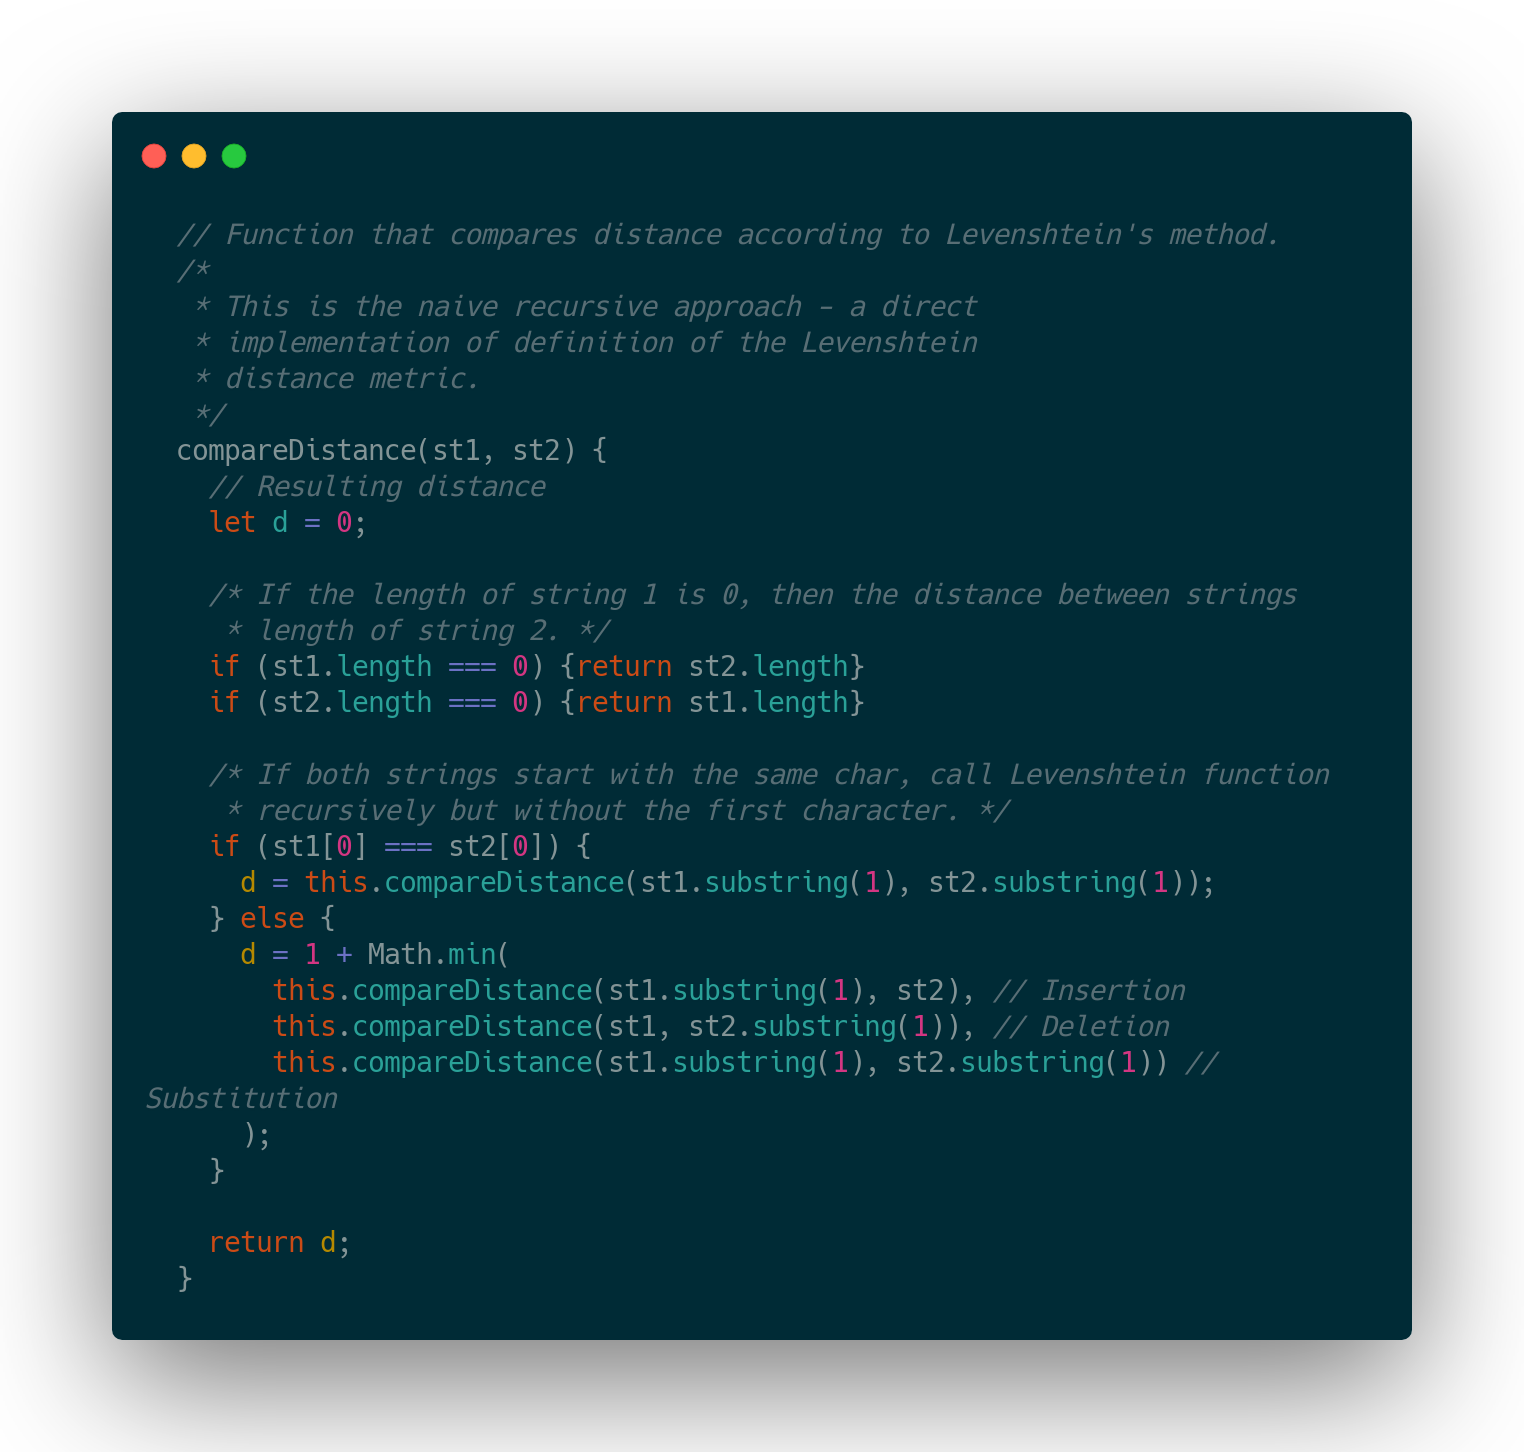
\includegraphics[scale=0.25]{recursive.png}
\end{figure}

Działanie tego algorytmu kończy się, gdy długość
jednego lub obydwu słów spadnie do 0. \cite{jlordiales::edit}

Niestety ta implementacja nie jest zbyt wydajna.
W związku z tym, że ten algorytm tworzy "'drzewko decyzji"' i
oblicza wynik dla każdego ciągu znaków który znajduje się w
tym drzewku, wykonuje on bardzo dużo niepotrzebnych operacji, co
zwiększa jego złożoność czasową.

Druga implementacja pokazuje, że ten algorytm da sie zoptymalizować
przy użyciu programowania dynamicznego.

\subsection{Implementacja wykorzystująca programowanie dynamiczne}
Programowanie dynamiczne polega na rozbiciu
większego problemu na mniejsze "'podproblemy"' i
stopniowe rozwiązywanie tych "'podbroblemów"'
aż główny problem stanie się na tyle trywialny, że jego rozwiązanie
będzie wystarczająco proste.

Poniżej znajduje się program wykorzystujący programowanie
dynamiczne w celu znalezienia odległości Levenshteina.

\begin{figure}[H]
    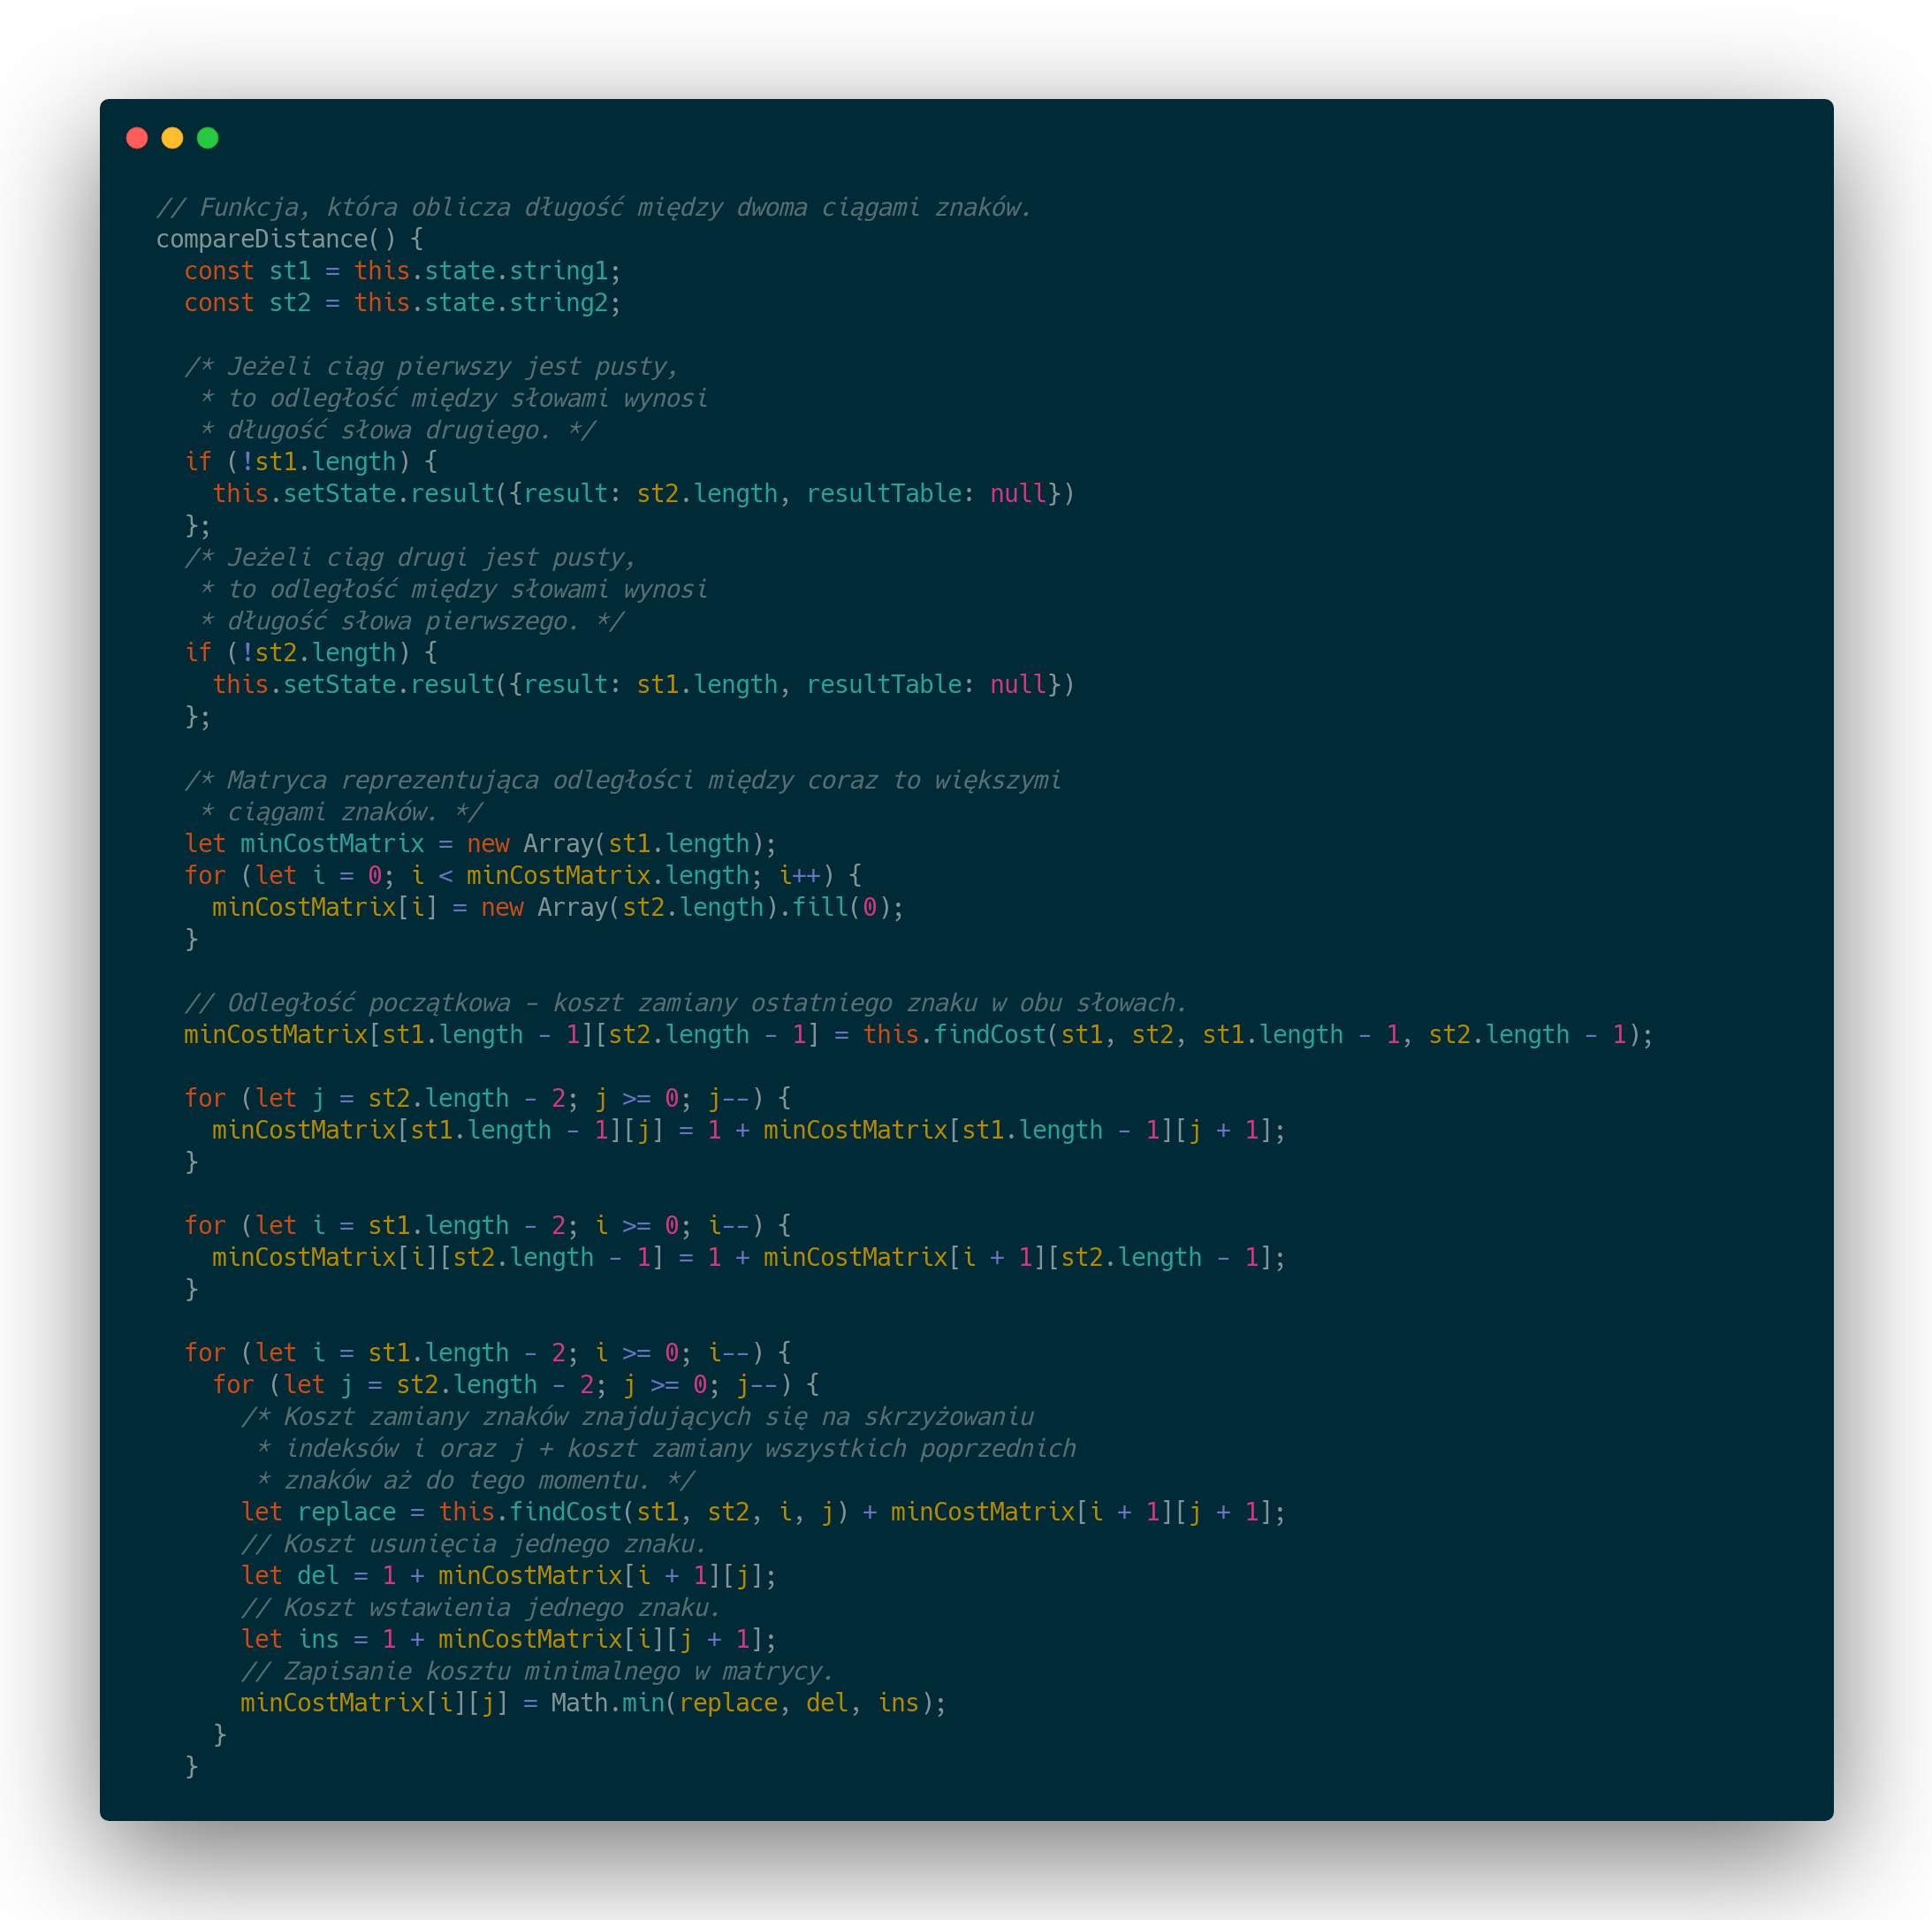
\includegraphics[scale=0.17]{dynamic.png}
\end{figure}

Algorytm tworzy "'matrycę"' zawierającą najniższe koszty wybrane
z pośród trzech operacji. Program, który stworzyłem przedstawia
te koszty w formie tabeli.

Obydwa programy zamieściłem jako strony internetowe GitHub pages.
Można dzięki nim porównać prędkość obliczania odległości Levenshteina
w implementacji rekursywnej i programowania dynamicznego.

\bibliographystyle{plain}
\bibliography{references}
\end{document}